\Chapter{Gesztusok}

\Section{Felismerendő gesztusok}

A szoftver használata közben a prezentáló személy különféle gesztusok segítségével léphet kapcsolatba a virtuális elemekkel. Általában a felhasználó a karjai mozgatásával valósítja meg ezeket a mozdulatokat.

\begin{itemize}
\item \textbf{Sweep}: Egyenes vonalú mozgás. A mozgásnak van iránya és két képkocka között megfigyelhető a hossza is.
\item \textbf{Shift}: Bizonyos virtuális elemek közvetlenül is reagálnak a környezetükben történő mozgásra. Az ilyen elemek az irányukba történő mozgással megegyező irányú mozgással reagálnak. Vagyis a prezentáló személy például a kezei segítségével egyszerűen eltolhatja az adott virtuális elemet.
\item \textbf{Blink}: Az ujjak gyors ökölbe zárása vagy a tenyér széttárásának mozdulata.
\item \textbf{Drag}: Bizonyos virtuális elemeket a prezentáló személy képes megfogni, majd odébbhúzni és elengedni. A funkció eléréséhez a prezentálónak egy \textit{Blink} gesztust kell végrehajtania. Az elkapás pillanatában az adott objektum a \textit{Blink} pozíciójára (a prezentáló kézfejére) tapad és követi annak helyzetét. A felhasználó így tetszőleges irányba mozgathatja az "elkapott" elemet. Egy újabb \textit{Blink} gesztussal pedig a kívánt helyére teheti azt.
\item \textbf{Rotation}: A videófolyamon történő örvénylő mozgás, ami akár több ponton is megfigyelhető. Ez lehet például karlendítés, körvonal/ív menti mozgás, tenyerek forgatása.
\item \textbf{Többpontos kezelés}: A képen lévő összefüggő, nagyobb elmozdulások keresése, \textit{Blob}-ok alapján. Több pont egymáshoz képesti vizsgálata különféle szempontok alapján.
\end{itemize}

\Section{Képek és vektor mezők}

Az elmozdulás becslésére az ún. \textit{Motion-Flow} technikák tűntek a legalkalmasabbnak. Egy kiemelkedő és széles körben elterjedt eljárás a Bruce D. Lucas és Takeo Kanade által kidolgozott módszer, melynek implementálása az \textit{OpenCV}-ben is megtalálható.

A Lucas-Kanade dedikált pontok követésére hivatott. Segítségével meghatározható a videófolyamon történő mozgás. Ehhez képkockapárokat kell összehasonlítani a kijelölt pont(ok) szemszögéből. A módszer azon a megállapításon alapszik, hogy a videófolyamon egy kijelölt pont és a körülötte lévő pixelek halmaza közel azonos intenzitású a vizsgált időintervallumban. Ha  a ponthoz tartozó valós idejű objektum elmozdul a korábbi helyzetéről és az általa képviselt új pont a vizsgálandó pont bizonyos tartományába esik, akkor a módszer képes becslést adni a pont új helyzetére a videófolyamon. A módszer használatánál feltételezzük azt is, hogy a videófolyamon megfigyelhető mozgás viszonylag lassú, vagyis két képkockát vizsgálva az új pont nem eshet kívül a vizsgált pont tartományából. A módszer tetszőleges pontok halmazára alkalmazható.

Az \textit{OpenCV}-ben található implementáció ún. \textit{kép-piramis}-ok használatával próbálja kiküszöbölni a nagy mozdulatok esetén fellépő hibás eredményeket, vagyis a vizsgálandó képeknek különböző felbontású változatait vizsgálja iteratívan a kisebb felbontástól az eredeti felbontásig haladva. A piramis mélysége tetszőleges, a legkisebb szint egyetlen pixelből is állhat. Kis felbontások mellett a nagyobb mozdulatok könnyebben azonosíthatóak, a piramis szélesebb szintjeihez közelítve, nagyobb felbontások mellett pedig pontosítódik a becslés. 
A módszer elsősorban szürkeárnyalatos képekre használatos, mivel az intenzitás értékek ilen esetekben jóval konzisztensebbek, de megfelelő paraméterek megválasztása mellett színes képekre is alkalmazható. \cite{bradski2008learning} 

\cite{lucas1981iterative} 
\textit{Flow Motion} működésének a leírása a cikk alapján...\\
Elmozdulás becslésének módja...\\
Részletezés képletekkel, ábrákkal...\\
Néhány képlet az \textit{OpenCV} dokumentációjából kimásolva:
% https://docs.opencv.org/4.1.1/d4/dee/tutorial_optical_flow.html
\begin{align*}
I(x,y,t) = I(x+dx,y+dy,t+dt)
\end{align*}
\begin{align*}
f_xu+f_yv+f_t=0
\end{align*}
\begin{align*}
f_x = \frac{\partial f}{\partial x} &; f_y = \frac{\partial f}{\partial y}\\
u = \frac{dx}{dt} &; v = \frac{dy}{dt}
\end{align*}
\begin{align*}
\bmatrix u \\ v \endbmatrix = {\bmatrix {\sum_{i}f_{x_i}}^2 & \sum_{i}f_{x_i}f_{y_i}\\ \sum_{i}f_{x_i}f_{y_i} & {\sum_{i}f_{y_i}}^2 \endbmatrix}^{-1} \bmatrix -\sum_{i}f_{x_i}f_{t_i} \\ -\sum_{i}f_{y_i}f_{t_i} \endbmatrix
\end{align*}

A módszer \textit{Spare Optical-Flow}-t valósít meg, vagyis egymástól különálló pontokat vizsgál, ellentétben a \textit{Dense Optical-Flow} módszerekkel, melyek a teljes kép vizsgálatával számolják ki az elmozdulás vektorokat. (forrás) Az utóbbi módszerek számításigénye kifejezetten magas. Valós idejű alkalmazás esetén problémákba ütközhetünk gyengébb hardverek esetében. A mozgás valós idejű detektálására a \textit{Spare Optical-Flow} módszerek is kielégítő eredményekkel szolgálnak, néhány trükk alkalmazása mellett. Ilyenek például a fent említett \textit{kép-piramisok} használata a gyors mozgások pontos követésére és a vizsgálandó pontok kijelölésének a stratégiája is. A pontok kijelöléséhez egy rácsszerkezetet gondoltam a legmegfelelőbbnek, ahol a pontok a rács metszéspontjaiban helyezkednek el. A képtartományt ily módon egyenletesen tudjuk lefedni.

\Section{Rácspontok kezelése}

Az \textit{Optical-Flow} eljárást tetszőleges számú pontra elvégezhetjük. Ha létrehozhatunk egy rácsszerkezetet fix pontokkal, akkor a képtartományt egyenletesen lefedhetjük a pontok halmazával.
Ezen pontokat felhasználva minden iterációban az éppen aktuális és az egyel korábbi szürkeárnyalatos képkockákra elvégezhetjük az eljárást és így minden esetben kapunk egy új ponthalmazt, amely az eljárás eredménypontjait tartalmazza. Az eredeti és az új pontokból egy vektormezőt kapunk.

\begin{figure}[h]
\centering
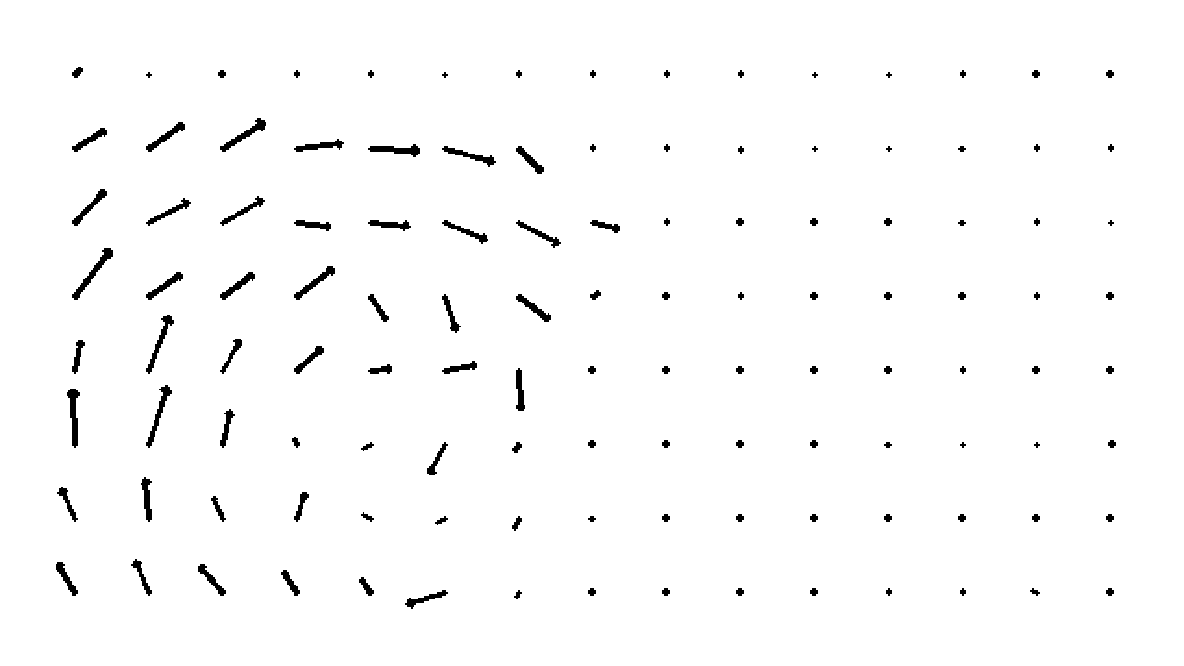
\includegraphics[width=11.2truecm, height=6.3truecm]{images/vectorField_screenshot.png}
\caption{Képernyőfotó a vektormezőről}
\label{fig:vectorfield}
\end{figure}

A mozgás detektálása rácspontok segítségével kevesebb számítást igényel, mintha minden pixel elmozdulását vizsgálnánk és az elmozdulás becslésére is elfogadható eredményeket kapunk.
A rács sűrűségét tetszőlegesen megadhatjuk. Minél sűrűbb a rács szerkezete, annál több pontot vizsgál a szoftver, ami nagyobb pontosságot is eredményez. Viszont a sűrűbb rács használata a futási időt is befolyásolja. Egy gyengébb hardver esetén nem ajánlott magas sűrűség értékkel futatnunk a programot, mivel tapasztalataim szerint jelentős lassulásra számíthatunk.

A rácspontok helyzetének meghatározásához elsősorban definiálnunk kell egy sűrűségi változót. A sűrűség-értéknek kettő-hatványának kell lennie, hogy a négyzetes rácsszerkezet pontosan illeszkedjen a videófolyam képkockáira, amelyek képaránya általában 16:9-es vagy 4:3-as lehet. A videófolyam felbontása forrásonként változhat. Hasonló képarányok esetében minden esetben azonos mennyiségű pontot generálhatunk, ha a pontok közötti távolságot, vagyis a \textit{lépésközt}, a képkocka felbontásának és a rácssűrűségnek a függvényében határozzuk meg.
\begin{align*}
\textit{lépésköz} = \frac{\textit{szélesség}}{\textit{sűrűség}}
\end{align*}
, ahol a \textit{szélesség} a képkocka szélessége pixelekben mérve.\\
A \textit{lépésköz} érték segítségével határozhatjuk meg a pontok helyzetét.\\
\newline
\noindent \textbf{Rácspontok$\_$generálása}(szélesség, magasság, lépésköz, @rács)\\ 
\textbf{FOR} i $\leftarrow$ lépésköz \textbf{TO} (magasság/lépésköz)-1 \textbf{DO}\\
\indent \textbf{FOR} j $\leftarrow$ lépésköz \textbf{TO} (szélesség/lépésköz)-1 \textbf{DO}\\
\indent \indent rács $\leftarrow$ rács.append([j,i])\\
\textbf{RETURN} rács

\Section{Hőtérkép}

A vektormező egyes pontjait vizsgálva szerkeszthetünk egy ún. \textit{Hőtérkép}-et, amelyben különböző intenzitásértékekkel jelöljök az egyes vektorok hosszait. A \textit{Hőtérkép} egy $n*m$-es mátrix, ahol $n$ a vektormező sorainak, $m$ pedig az oszlopainak a száma. A \textit{Hőtérkép} minden eleme egy BGR (blue, green, red) hármas értékkel van ellátva. Ezen értékek jelölik az egyes elemek színét.\\
Az értékek a következőképpen kerülnek kiszámításra:\\
\newline
\noindent \textbf{Hőtérkép$\_$kiszámítása}(@vektormező, érzékenység, @hőtérkép)\\ 
Input paraméter: vektormező (n*m-es mátrix), érzékenység\\
Output paraméter: hőtérkép\\
\textbf{FOR} i $\leftarrow$ 1 \textbf{TO} Hossz(vektor$_n$) \textbf{DO}\\
\indent \textbf{FOR} j $\leftarrow$ 1 \textbf{TO} Hossz(vektor$_m$) \textbf{DO}\\
\indent \indent hőérték$_{ij}$ $\leftarrow$ hossz(vektor$_{ij}$)*érzékenység\\
\indent \indent \textbf{IF} hőérték$_{ij}$ > 255\\
\indent \indent \indent \textbf{THEN} hőérték$_{ij}$ $\leftarrow$ 255\\
\indent \indent hőtérkép$_{ij}$ $\leftarrow$ (255-hőérték$_{ij}$, 0, hőérték$_{ij}$)\\
\textbf{RETURN} hőtérkép\\
\newline
0 pixel hosszúság esetén az adott indexű elem (255, 0, 0) értéket kap, vagyis kék színnel jelöljük. Ha egy adott vektor számított hőértéke eléri a 255-öt, a hozzá tartozó \textit{hőtérkép-érték} (0, 0, 255) intenzitásértéket kap, vagyis tiszta piros színnel fog megjelenni.
A \textit{érzékenység} értékkel állíthatjuk be, hogy mely vektorhosszakat vegyen a program figyelembe. Az érték megadja, hogy milyen mértékű legyen a vektorok nagyítása, befolyásolva ezzel a számított \textit{hőértéket}.

\begin{figure}[h]
\centering
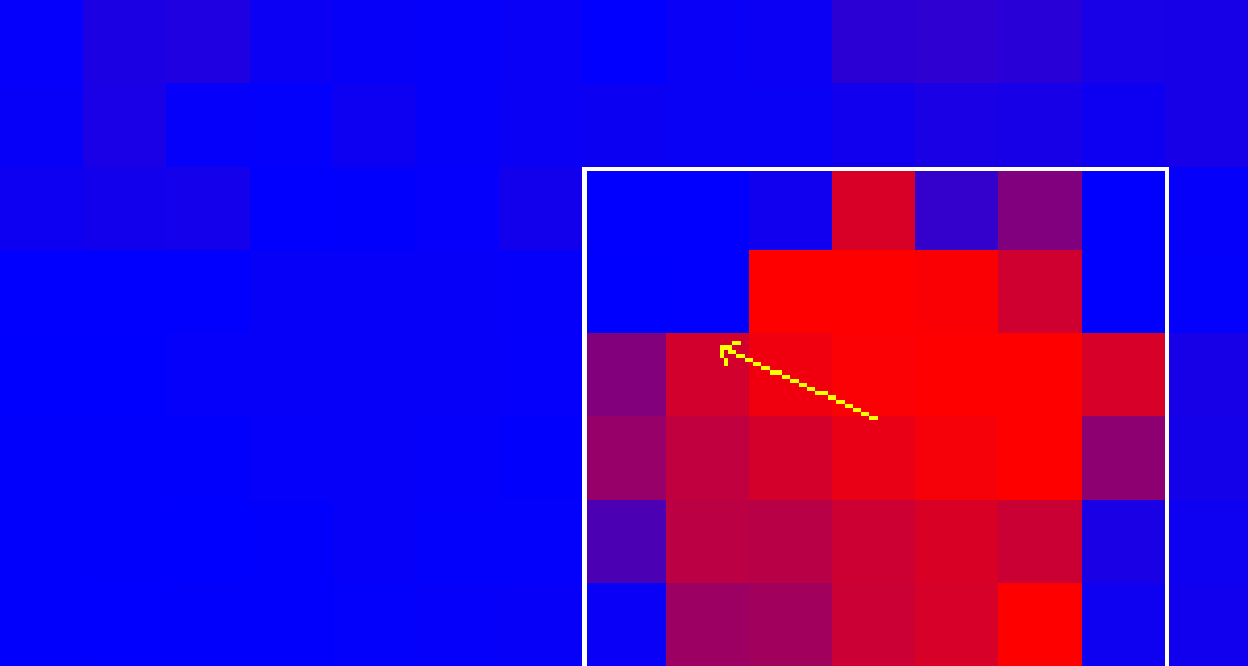
\includegraphics[width=11.2truecm, height=6.3truecm]{images/HeatMap_screenshot.png}
\caption{Képernyőfotó a hőtérképről}
\label{fig:heatmap}
\end{figure}

Az így kapott mátrixból ezután különféle információkat nyerhetünk ki. Az intenzitás értékeket vizsgálva meghatározhatjuk a nagyobb elmozdulások csoportjait. Ehhez küszöbölni kell a mátrixot, majd a kapott képen kontúrok kereséssel meg lehet állapítani, hogy mely vektorok tartoznak egy csoportba. A \ref{fig:heatmap} ábrán megfigyelhető, hogy az összetartozó értékek fehér kerettel van jelölve. Továbbá az ábrán sárga nyílakkal vannak jelölve az elmozdulások irányai. A csoportokat külön-külön vizsgálva tehát további értékes információkhoz juthatunk. Ilyen például az egyes csoportok iránya is, amelyet egy lokális eredővektor számításából kaphatunk meg. A csoportokat felhasználhatjuk további funkciók megvalósítására is, mint például a \textit{Többpontos kezelés} vagy a \textit{Rotation} vizsgálatára is.

\Section{Kontrollpontok és vektorok számítása}

\SubSection{Sweep}

A \textit{Sweep} gesztus két tulajdonsággal írható le: A mozgás irányával és hosszával. A mozgás irányát egy $\vec{v}\in\Bbb R^2$ irányvektorral határozhatunk meg, amelyet a \textit{vektormező} globális eredővektoraként kapunk meg.
\begin{align*}
  \vec{v} = \sum_{i=1}^n\vec{u_i}
\end{align*}
, ahol $\vec{u}$ a teljes képre vett vektormező vektorai.\\
A mozgás hossza a vektormező vektorainak átlagos hosszában mérhető és pixelszámban fejezhető ki.
\begin{align*}
  \overline{x}=\frac{\sum_{i=1}^n \left|\vec{v_i}\right|}{n}
\end{align*}
, ahol $n$ a vektormező vektorainak a száma.

\begin{figure}[h]
\centering
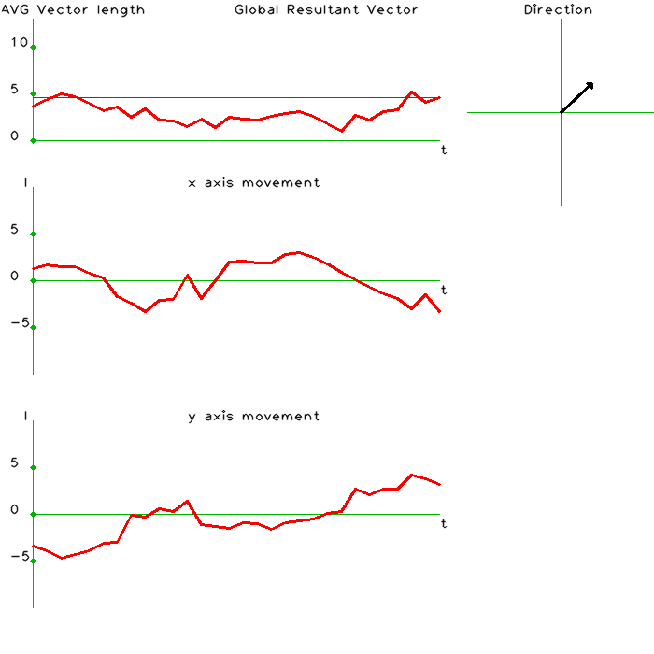
\includegraphics[width=11.86truecm, height=5truecm]{images/ResultantPlot_screenshot.png}
\caption{Képernyőfotó a globális eredővektor grafikonjáról}
\label{fig:resultantplot}
\end{figure}

Az ábrán megfigyelhető a globális eredő vektor hosszainak változása egy 30 képkockás \textit{csúszóablakban} és az éppen aktuális irányvektor is.

\SubSection{Shift}

A \textit{Shift} tulajdonsággal rendelkező virtuális elemeknek mindig van egy aktuális pozíciójuk $(x,y)$, szélességük és hosszuk $(w,h)$, illetve sebesség értékük $v_{xy}$ a két tengelyre vonatkozóan.

A \textit{Shift} viselkedésének meghatározásához első lépésként az adott virtuális elem területére eső vektorokból $\vec{v}_l$  lokális eredővektort számolunk. Az elem területére eső vektorok és a lokális irányvektor meghatározható az elem pozíciója és a mérete alapján a következő módon:
\begin{align*}
  (i_1, j_1), (n, m) &= \lfloor \frac{(x,y),(w,h)}{\textit{rács lépésköze}} \rfloor\\
  \vec{v_l} &= \sum_{i=i_1}^n \sum_{j=j_1}^m \vec{u}_{ij}
\end{align*}
Az eredővektorból ezután irányvektort számolunk. Majd az irányvektok segítségével kiszámoljuk az elem sebességét:
\begin{align*}
  v_{xy} = v_{xy} + \frac{\vec{v}_l}{(n*m)}*\textit{gyorsulás}
\end{align*}
, ahol $\textit{gyorsulás} > 0$.\\
Az elem pozíciója $(x,y)$ a sebesség függvényében változik.
\begin{align*}
  (x,y) = (x,y)+v_{xy}
\end{align*}
A sebesség értéket minden iteráció végén tompítani kell, hogy a kezelt virtuális elem meg tudjon állni egy bizonyos ponton. Ha az adott elemet nem éri tovább erő, akkor a tompítás lassulást eredményez, a sebesség csökkenni fog. Olyan hatást is el tudunk érni egy helyesen megválasztott értékkel, mintha az eltolás után az elem csúszós felületen mozogna és így fokozatosan lassul le az iterációk során.
\begin{align*}
  v_{xy} = v_{xy}*\textit{tompítás}
\end{align*}
, ahol $0 \leq \textit{tompítás} < 1$

% Ide még lehet jöhetne majd egy szemléltető képernyőkép, vagy valami ábra...

\SubSection{Drag}

A \textit{Drag} az elem elkapása utáni állapot jelenti, amikor a felhasználó az elkapott elem helyzetét szabadon változtathatja, majd új pozíciójára teheti. Ennek a funkciónak a megvalósításához többféleképpen is hozzáláthatunk.

Az első ötletem szerint a vektormező vektorait felhasználva lokális eredővektorokat számolva becsülte volna meg a program a mozgatandó virtuális elem új helyzetét. Ez a megoldás gyakorlatban az elvárásokat nem elégítette ki. Több probléma is adódott ezzel a megoldással. A \textit{Rács} lyukacsossága miatt nem mindig esett vizsgálandó pont a mozgás helyére. Az egyes kiugró értékek is befolyásolták a végeredményt, a mozgatandó elemek ilyen esetekben gyorsabban mozogtak a vártnál. Ez a megoldás tehát nem tűnt stabilnak, a vektormező rácsának sűrítésével pedig a program jelentős lassulásba ütközött volna. Más megoldás után kellett kutatni.

Mivel a \textit{Drag}-et előreláthatólag a prezentáló csak rövid időszakaszokban fogja használni, ezért a következő ötlettel áltam elő: a \textit{Blink} gesztus pozíciójára kontollpont(okat) illeszthetnénk, melyekre külön-külön elvégezhetnénk az \textit{Optical-Flow} eljárást és a pont vagy a pontok súlypontjának pozíciója függvényében változna a mozgatandó virtuális elem pozíciója is. Már egyetlen kontrollpont használata is kielégítő eredményt adott. Több kontrollpont használata csupán csak a biztonság érdekében tűnik megfelelőnek. Ha esetleg egy pont új pozícióját rosszul becsülné meg az eljárás és a pont egy bizonyos ponton leragadna, akkor maradjanak olyan "tartalék" pontok is, amelyek a funkció helyes működését biztosítani tudják.

\SubSection{Blink}

A \textit{Blink} gesztusok felismerésére először egy ún. \textit{Frame differencing} technikát kell alkalmaznunk.
Ehhez a videófolyam aktuális képkockájának és az egyel korábbi képkockájának abszolút különbségét kell meghatározni, majd az így kapott képen küszöbölést kell végrehajtani. Eredményképp egy olyan képet kapunk, amelyen az elmozdulás figyelhető meg fehér színnel jelölve. A keletkezett képen különféle alakzatok alakulhatnak ki. Az egyes mozdulatok hasonló nyomot hagynak maguk után. Így tehát egy \textit{Blink} mozdulat leadásakor jellegzetes mintázat rajzolódik ki.

Tervek, ötletek ezzel kapcsolatban...

\SubSection{Rotation}

A \textit{Rotation} gesztus két tulajdonsággal íható le: ezen gesztusnak mindig létezik egy elméleti középpontja, ami körül történik az elmozdulás, valamint van iránya is.
Becslést adni a mozgás lehetséges középpontjának pozíciójára a vektormező elemzésével célszerű.
A vektorokhoz egyenes egyenleteket szerkeszthetünk. Az egyenes egyenletének egy pontja a vektot kezdőpontja lesz, a normálvektora pedig az egyenes irányvektora.

Két egyenletből álló egyenletrenszer megoldásaként megkapjuk az $x,y$ ismeretlen értékeket, melyek a két egyenes metszéspontjának a pozícióját adják meg.
A metszéspontokat számolva létrejön egy ponthalmaz, amelynek súlypontja az elméleti középpont közelében fog elhelyezkedni.
A programom \textbf{jelenleg} csupán a szomszédos vektorok egyenleteit oldja meg, ezzel számítási időt spórolva meg, kedvező futási időt biztosítva. A becslés pontossága viszont romlani fog.

Ha pedig több \textit{Rotation} pontot is vizsgálni szeretnénk, akkor segítségül hívhatjuk a \textit{Hőtérkép}-ből kinyert vektorcsoportok halmazait, majd ezen csoportokon külön-külön elvégezhetjük az eljárást a lokális súlypontok után kutatva.

\SubSection{Többpontos kezelés}


Irányok esetében $\vec{u},\vec{v}\in \Bbb R^2$ esetén
\begin{align*}
\vmatrix \vec{u}+\vec{v} \endvmatrix &< \varepsilon_{\text{irány}}\\
&\approx \vec{0}
\end{align*}
